\documentclass{mwart}
\usepackage{multicol}
\usepackage{polski} % Pozwala na użycie polskiego. Ustawia między innymi fontenc na T1
\usepackage[utf8]{inputenc} % Informuje o kodowaniu
\usepackage{enumitem}
\usepackage{xcolor}
\usepackage{xcolor}% http://ctan.org/pkg/xcolor
\usepackage{hyperref}
\usepackage{listings}
\usepackage{float} % Ustawianie obrazów
\usepackage[caption = false]{subfig} % Wiele obrazów w jednej figurze
\definecolor{LinkColor}{HTML}{1d5cc1}
\renewcommand{\labelitemi}{\textbullet} % Zmiana symbolu wliczeń

\lstset{
  basicstyle=\ttfamily,
  columns=fullflexible,
  breaklines=true,
  postbreak=\mbox{\textcolor{red}{$\hookrightarrow$}\space},
}

\definecolor{LinkColor}{HTML}{1d5cc1}

\usepackage{tabto}

\usepackage{graphicx} % Pakiet do obrazów
\graphicspath{ {./Obrazy/} } % Folder, z którego będą brane obrazy

% Nie twórz nowych stron
\usepackage{etoolbox}
\makeatletter
% \patchcmd{\chapter}{\if@openright\cleardoublepage\else\clearpage\fi}{}{}{}
\makeatother

\newcommand{\paragraphnl}[1]{\paragraph{#1} \mbox{} \\} % Paragraf z nową linią

\title{Projekt indywidualny ----  Raport końcowy}
\author{Krzysztof Dąbrowski}
\date{\today}

\begin{document}
\maketitle{}

\tableofcontents{}

% \section{Ostateczny projekt klas}

\section{Opis projektu}
Celem projektu jest napisanie aplikacji webowej pozwalającej na planowanie semestru studentom korzystającym z systemu \textit{USOS}.
W tym celu został wykonany program w języku C\# w oparciu o framework \textit{ASP.net MVC}. Dzięki temu możliwe było łatwe wydzielenie warstw widoku, modelu i kontrolerów.

Aplikacja została opublikowana w Internecie z wykorzystaniem chmury \textit{Microsoft Azure}.

\subsection{Wzorzec MVC}

\newpage{}
\section{Projekt klas}
\begin{figure}[H]
    \centering
    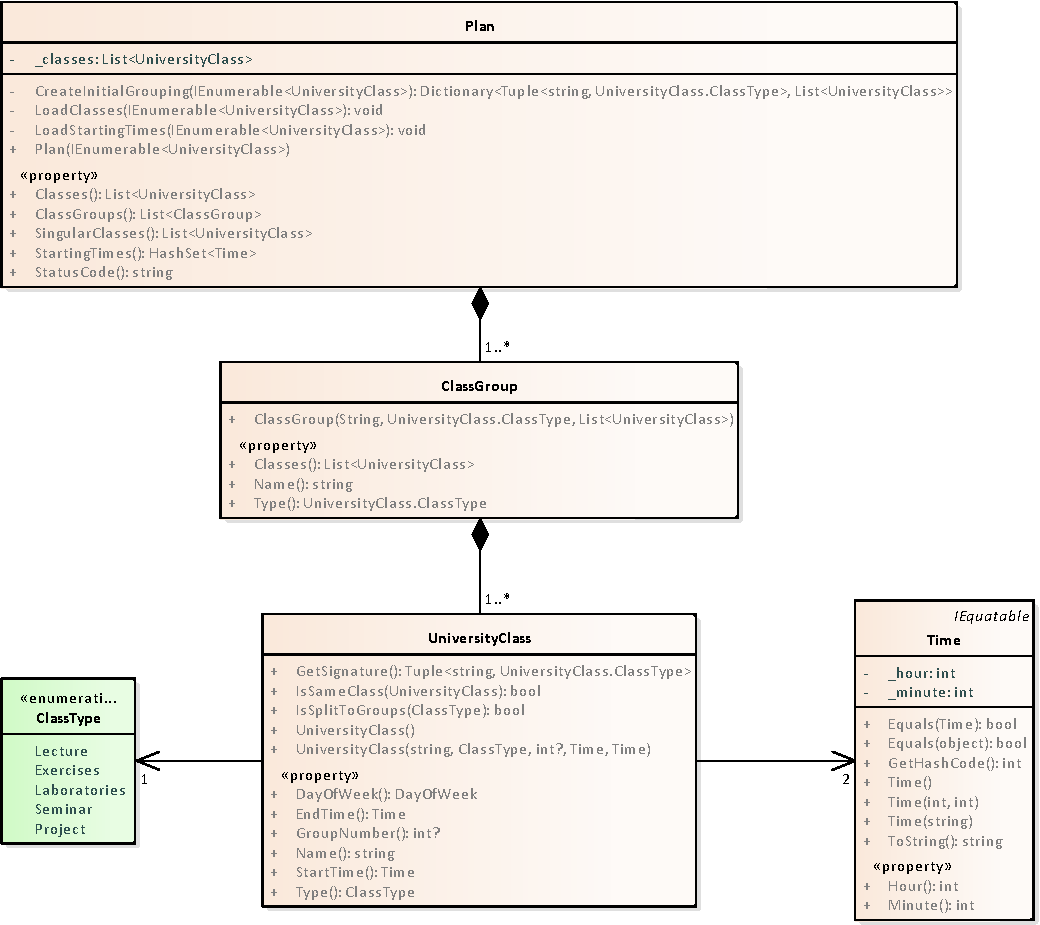
\includegraphics[width=13cm]{klasy.pdf}
    \caption{Modele}
    \label{}
\end{figure}

\section{Prezentacja działania}

\section{Opis użytych bibliotek}
linq
C\# JSON
jquery
knockout
bootstrap

\end{document}

